\documentclass{article}
\usepackage{bm}
\usepackage{amsmath}
\usepackage{graphicx}
\usepackage{mdwlist}
\usepackage[colorlinks=true]{hyperref}
\usepackage{geometry}
\usepackage{kotex}
\geometry{margin=1in}
\geometry{headheight=2in}
\geometry{top=2in}
\usepackage{palatino}
%\renewcommand{\rmdefault}{palatino}
\usepackage{fancyhdr}

%\pagestyle{fancy}
\rhead{}
\lhead{}
\chead{%
  {\vbox{%
      \vspace{2mm}
      \large
      Hardware System Design 4190.309A\hfill
\\
      Seoul National University
      \\[4mm]
      \textbf{Practice \#4. How to use IP catalog \& Synthesize}\\
      \textbf{Jiwon Lee, Sangjun Son}
    }
  }
}

%%%%%%%%%%%%%%%%%%%%%%%
\usepackage{xcolor}
\usepackage{listings}
\definecolor{vgreen}{RGB}{104,180,104}
\definecolor{vblue}{RGB}{49,49,255}
\definecolor{vorange}{RGB}{255,143,102}

\lstdefinestyle{verilog-style}
{
    language=Verilog,
    basicstyle=\small\ttfamily,
    keywordstyle=\color{vblue},
    identifierstyle=\color{black},
    commentstyle=\color{vgreen},
    numbers=left,
    numberstyle=\tiny\color{black},
    numbersep=10pt,
    tabsize=8,
    moredelim=*[s][\colorIndex]{[}{]},
    literate=*{:}{:}1
}

\makeatletter
\newcommand*\@lbracket{[}
\newcommand*\@rbracket{]}
\newcommand*\@colon{:}
\newcommand*\colorIndex{%
    \edef\@temp{\the\lst@token}%
    \ifx\@temp\@lbracket \color{black}%
    \else\ifx\@temp\@rbracket \color{black}%
    \else\ifx\@temp\@colon \color{black}%
    \else \color{vorange}%
    \fi\fi\fi
}
\makeatother

\usepackage{trace}
%%%%%%%%%%%%%%%%%%%%%%%

\usepackage{paralist}

\usepackage{todonotes}
\setlength{\marginparwidth}{2.15cm}

\usepackage{tikz}
\usetikzlibrary{positioning,shapes,backgrounds}

\begin{document}

\pagestyle{fancy}

\section*{Goal}

\begin{itemize*}
\item Implement base of Float32 multiplier + accumulator.
\item Implement Floating point / Integer fused multiply-adder using IP catalog.
\item Implement adder-array using accumulator module.
\end{itemize*}

\section{Implementation}

\subsection{Floating point fused multiply-adder}

이번 프로젝트는 IP catalog를 이용해보는 과제였기 때문에, 미리 구현된 floating point multiply-adder를 사용하고
testbench 에서 입력값을 조정하여 출력값을 확인하였다.
Verliog의 floating point representation은 IEEE 754 standard를 사용한다. 
즉, 32bit binary number는 다음과 같은 형태로 floating point로 전환된다. 
\begin{equation}
	 f = sign \times 2^{exponent} \times mantissa
\label{eqn1}
\end{equation}

IEEE 754의 부동소수점 표현은 크게 세 부분으로 구성되는데, 최상위 비트는 부호를 표시하는데 사용되며, 지수 부분 (exponent)과 가수 부분 (fraction/mantissa)이 있다~\cite{overton2001numerical}.
이를 시각적으로 나타내면 Figure~\ref{fig1} 같다.

\begin{figure}[ht]
	\centering
	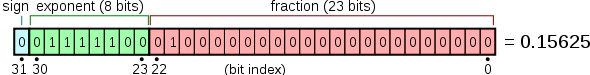
\includegraphics[width=0.7\textwidth]{fig/fig1.png}
	\caption{IEEE 754 single-precision binary floating-point format: binary32}
\label{fig1}
\end{figure}

결과값을 확인하기 위해 sign, exponent 그리고 mantissa 부분의 분포를 uniformly random 하게 만들기 위해서 Equation~\ref{eqn2}와 같은 범위 사이의 숫자를 뽑아 이어붙이는 식으로 입력값을 산정하여 test를 진행하였다.
\begin{equation}
	 sign \in [0, 2^1), \quad exponent \in [0, 2^8), \quad mantissa \in [0, 2^{23})
\label{eqn2}
\end{equation}
\begin{equation}
	 f = (sign \ll 31) + (exponent  \ll 23) + (mantissa)
\label{eqn3}
\end{equation}

위와 같은 방법으로 생성된 테스트 값들은 다음 Table~\ref{tab1}과 같다. 테스트에 사용된 입력값과 더불어 실험 결과값 또한 가시성을 높이기 위해 첨부하였다. IEEE 754의 모든 부분이 uniformly random 하게 선택되기 때문에 nan 또는 inf 값이 나올 수 있으며 해당 값에 따라 연산값이 바뀌는 것을 확인할 수 있다. 
\begin{table}[ht]
\renewcommand{\arraystretch}{1}
\begin{center}
\begin{tabular}{ |c | ccc | c |} 
 \hline
 $i$ & $a_{in}[31:0]$ & $b_{in}[31:0]$ & $c_{in}[31:0]$ & $res[31:0]$  \\ 
 \hline
1 & $-2.131260 \times 10^{23}$ 		& $4.226937 \times 10^{-22}$		& $-5.057321 \times 10^{-37}$	& -90.087020 \\
2 & $-9.676296 \times 10^{-24}$ 		& $-5.898969 \times 10^{20}$ 		& $-2.102489 \times 10^{14}$	& $-2.102489 \times 10^{14}$  \\ 
\vdots& & \vdots & & \vdots \\
10 & $-$nan  			& $-0.009755 $ 		& $-2.074778\times 10^{21}$							& $+$nan \\ 
19 & $-2.971665 \times 10^{25}$ 		& $-2.610150 \times 10^{15}$ 		& $-6.529525 \times 10^{-17}$	& $+$inf \\ 
\vdots& & \vdots & & \vdots \\
32 & $-6.609544 \times 10^{13}$ 		& $8.002746 \times 10^{-26}$ 		& $6.917540 \times 10^{35}$	& $6.917540 \times 10^{35}$  \\ 
 \hline
\end{tabular}
\caption{Abbreviated set of test inputs and outputs.}\label{tab1}
\end{center}
\end{table}

이미 존재하는 모듈을 활용해서 연산을 구현하고 올바른 값이 나오는 것을 확인할 수 있었다. delay가 존재하여 약 8 tu 뒤에 연산 결과가 나타나는 것을 관찰할 수 있었고 모듈마다 존재하는 catalog documentation을 통해 해당하는 설명을 찾을 수 있었다~\cite{fpmultiplyadder}. 아래 첨부된 결과를 통해 총 32개의 input과 output에 대한 waveform 양상을 파악할 수 있다.
\begin{figure}[ht]
	\centering
	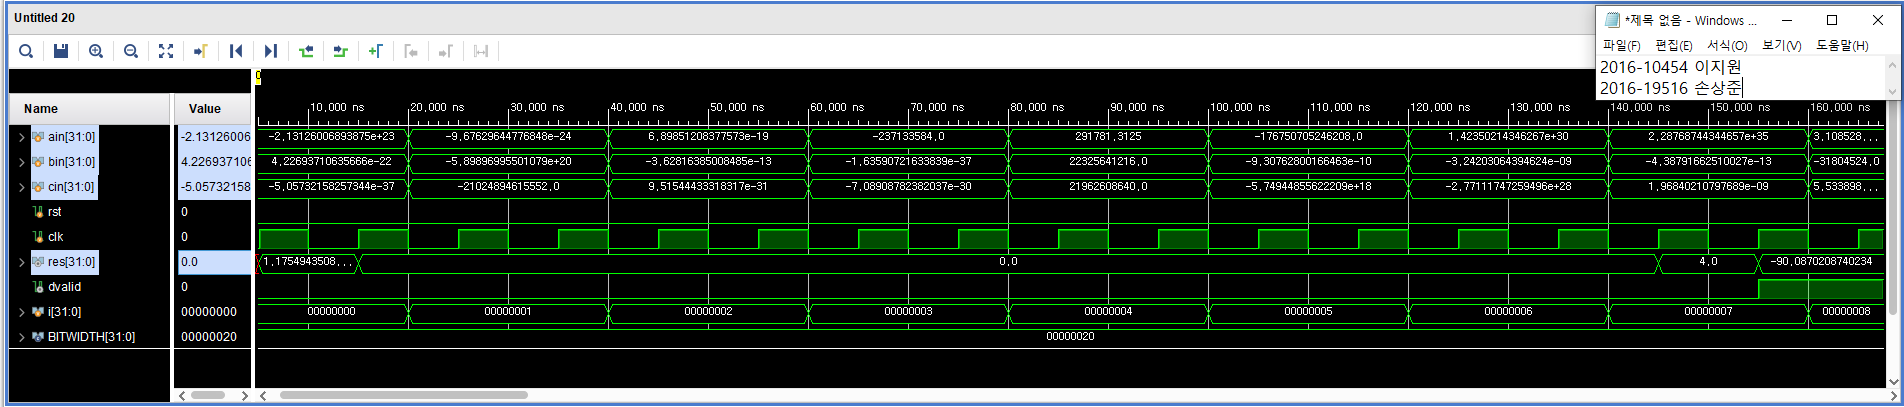
\includegraphics[width=1.0\textwidth]{../report/Waveform_32bit_FP_Multiply-Adder/tb_fp_muladd1.png}
	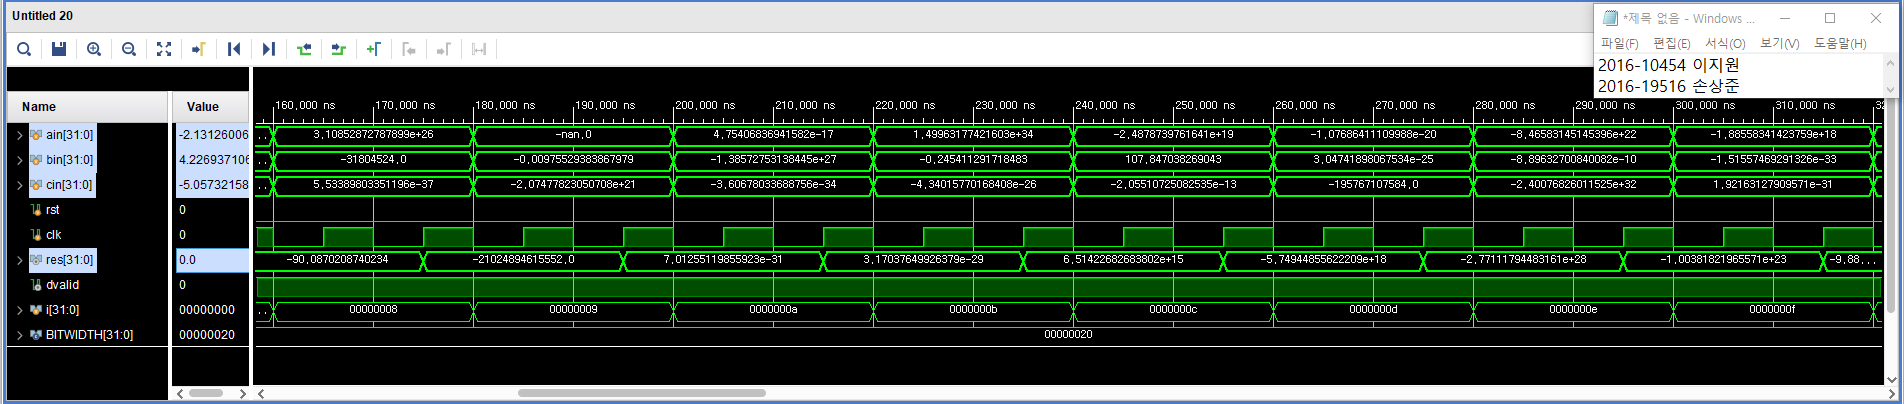
\includegraphics[width=1.0\textwidth]{../report/Waveform_32bit_FP_Multiply-Adder/tb_fp_muladd2.png}
	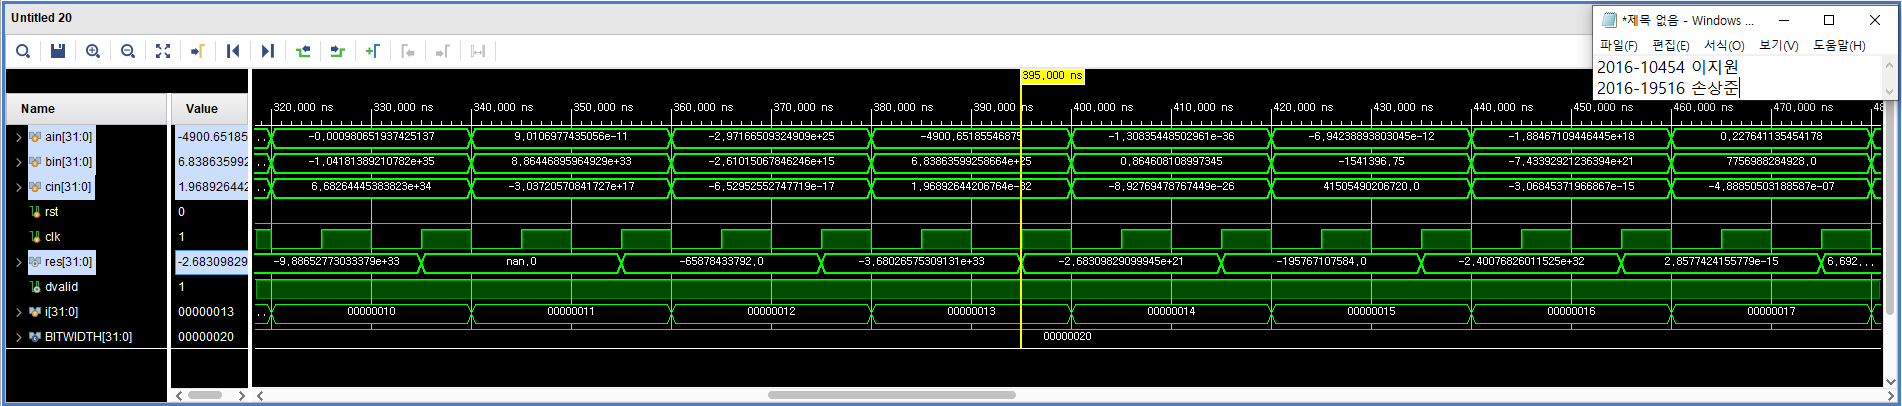
\includegraphics[width=1.0\textwidth]{../report/Waveform_32bit_FP_Multiply-Adder/tb_fp_muladd3.png}
	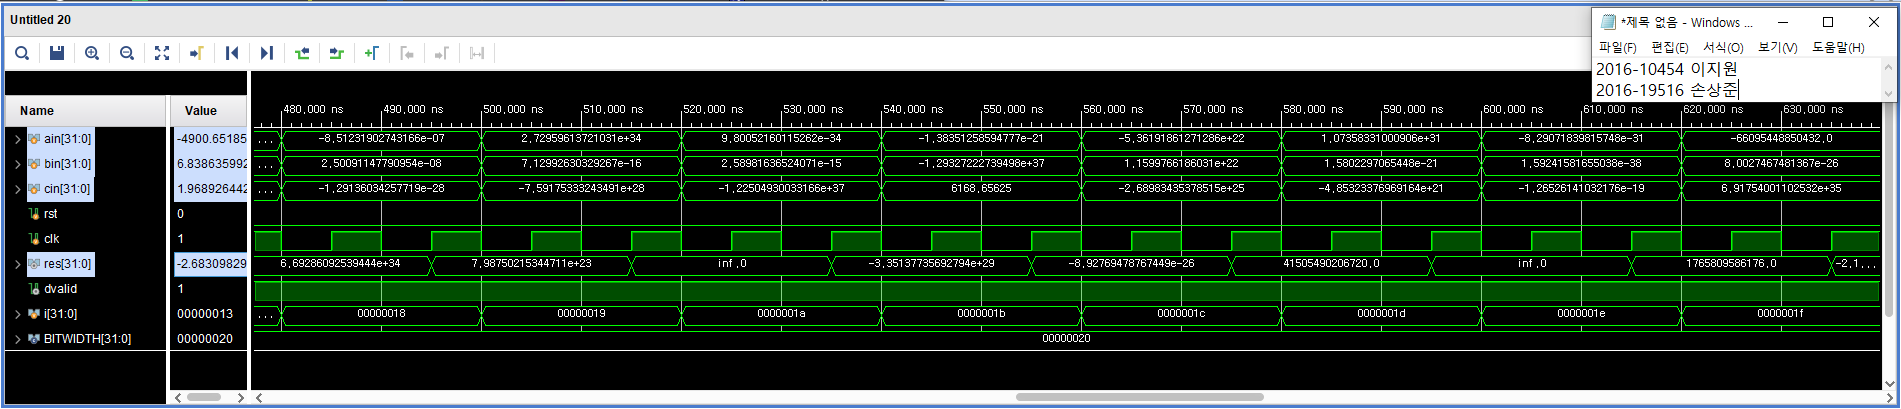
\includegraphics[width=1.0\textwidth]{../report/Waveform_32bit_FP_Multiply-Adder/tb_fp_muladd4.png}
\end{figure}
\begin{figure}[ht]
	\centering
	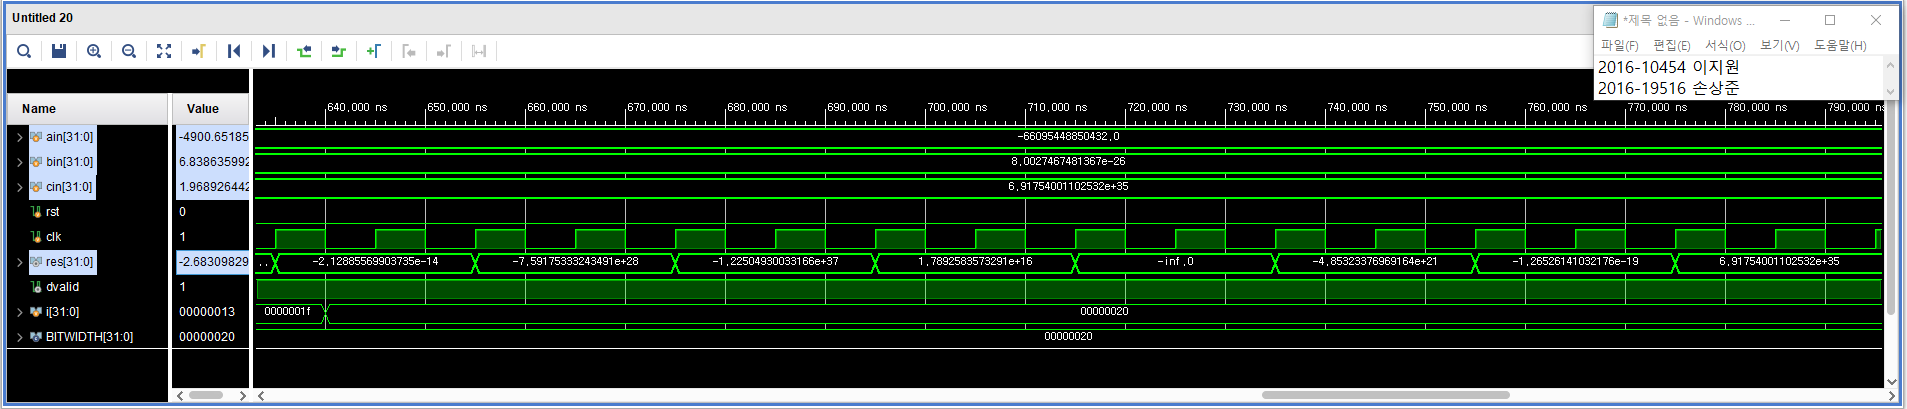
\includegraphics[width=1.0\textwidth]{../report/Waveform_32bit_FP_Multiply-Adder/tb_fp_muladd5.png}
\end{figure}

\subsection{Integer fused multiply-adder}
Floating point multiply-adder와 동일하게, 미리 구현된 IP catalog를 사용, testbench 에서 입력값을 조정하여 출력값을 확인하였다. 
IP catalog를 customize 할 때, Multiply와 Add가 동시에 수행되어 결과값을 나타내야 했기 때문에, P-A:B latency 와 P-C latency를 0으로 설정하였다. 

IP catalog에는 입력값에 clk signal이 존재하지 않았다. 따라서, async한 방식으로 A,B,C (inputs)의 값이 변화할 때, P (output)이 계산되는 것을 볼 수 있었다. 또한, P값이 나오기까지는 delay가 존재하였는데, 이는 주어진 A, B, C값을 최종 결과값으로 나타내기까지 걸리는 시간 (latency)이다.

\begin{figure}[ht]
	\centering
	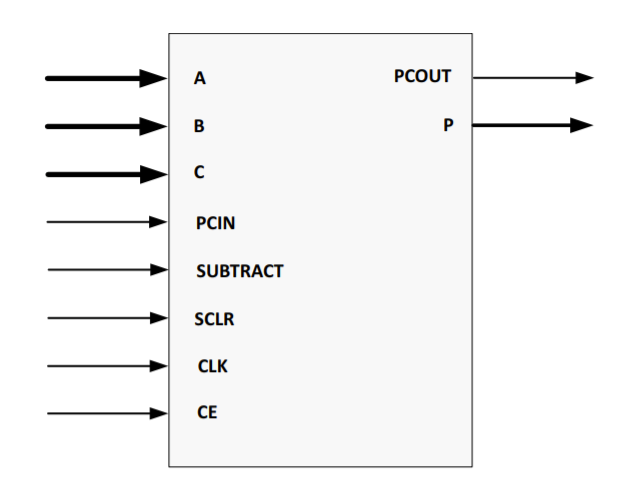
\includegraphics[width=0.5\textwidth]{fig/fig3.png}
	\caption{Representation of PG192 - Multiply Adder v3.0}
\label{fig3}
\end{figure}

위 Figure~\ref{fig3}는 우리 팀이 선정한 모듈인 integer fused multiply-adder의 전반적인 구조를 보여준다. 각각의 input/output port에 대한 기능 및 조건은 아래의 Table~\ref{tab2}과 같다. latency를 모두 0으로 설정함으로써 필요하지 않은 port는 생략하여 설명한다. 테스트벤치 결과는 FP fused multiply-adder와는 다르게 캡쳐결과와 연산 결과가 clk-synchronized 되어 있으므로 확인하기 쉬울 것이다.
\begin{table}[ht]
\renewcommand{\arraystretch}{0.9}
\begin{center}
\begin{tabular}{ |c | c | c |} 
 \hline
Name & I/O & Description \\ 
 \hline
A[31:0] &		Input		& 	A Input bus (multiplier operand 1)  \\
B[31:0] &	Input		&	B Input bus (multiplier operand 2)  \\
C[63:0] &		Input		& 	C Input bus (operand 1 of add/sub operation)  \\
SUBTRACT &		Input		& 	Controls Add/Subtract operation (High = subtraction, Low = addition)  \\
PCOUT &		Output		& 	Cascade Output   \\
P[63:0] &		Output		& 	Output bus \\
 \hline
\end{tabular}
\caption{Abbreviated set of test inputs and outputs~\cite{intmultiplyadder}.}\label{tab2}
\end{center}
\end{table}

\newpage
\begin{figure}[ht]
	\centering
	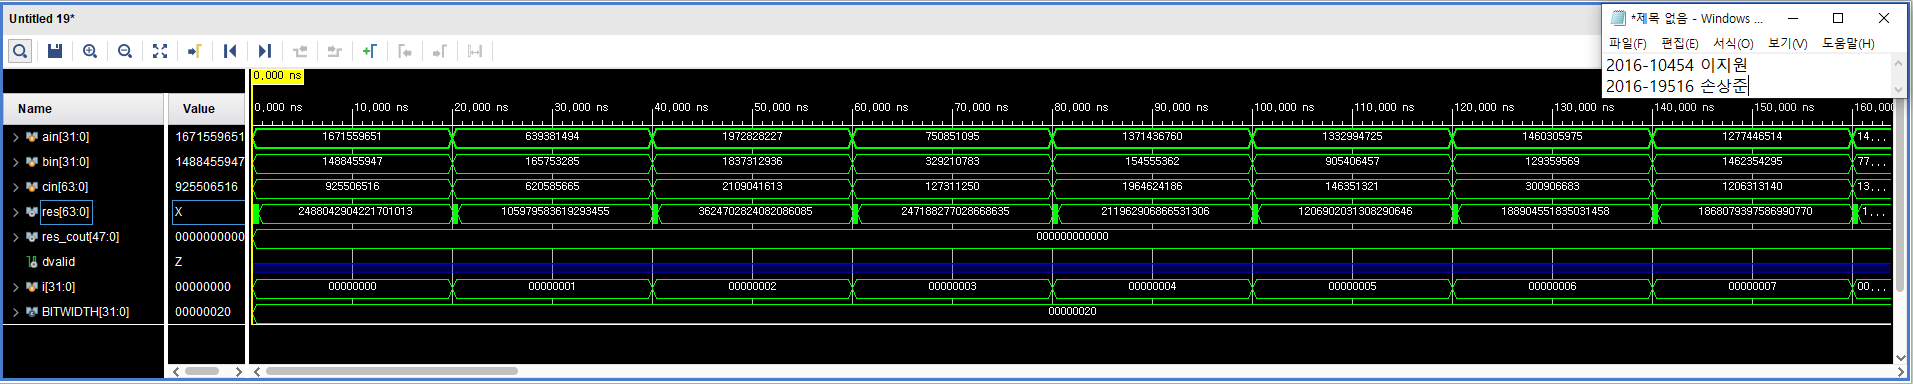
\includegraphics[width=1.0\textwidth]{../report/Waveform_32bit_Int_Multiply-Adder/tb_int_muladd1.png}
	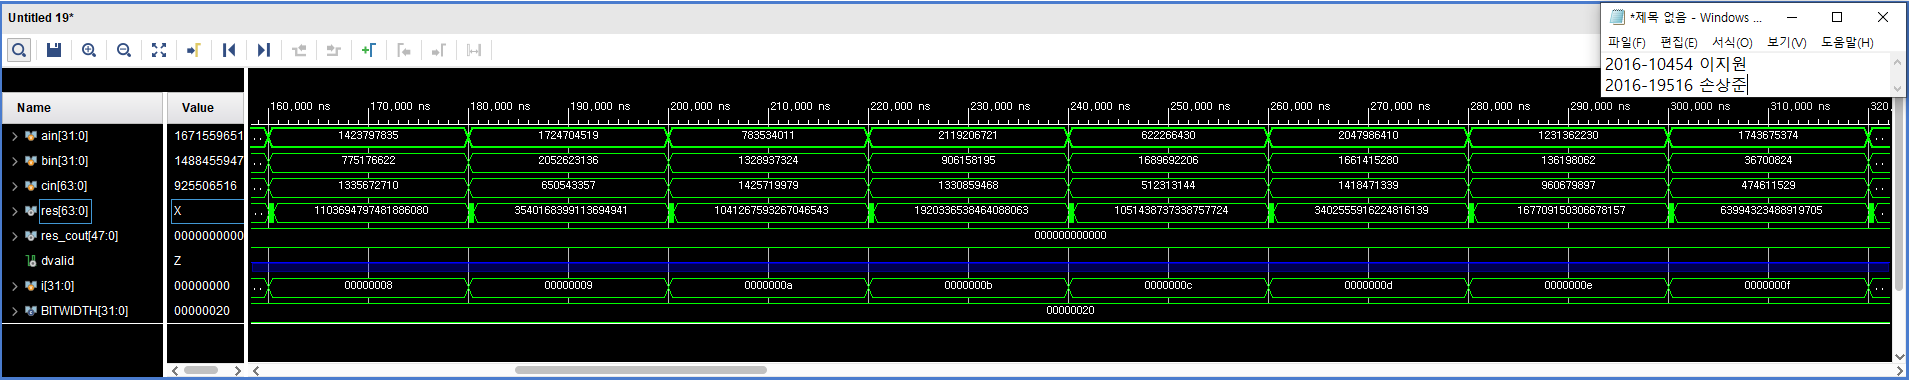
\includegraphics[width=1.0\textwidth]{../report/Waveform_32bit_Int_Multiply-Adder/tb_int_muladd2.png}
	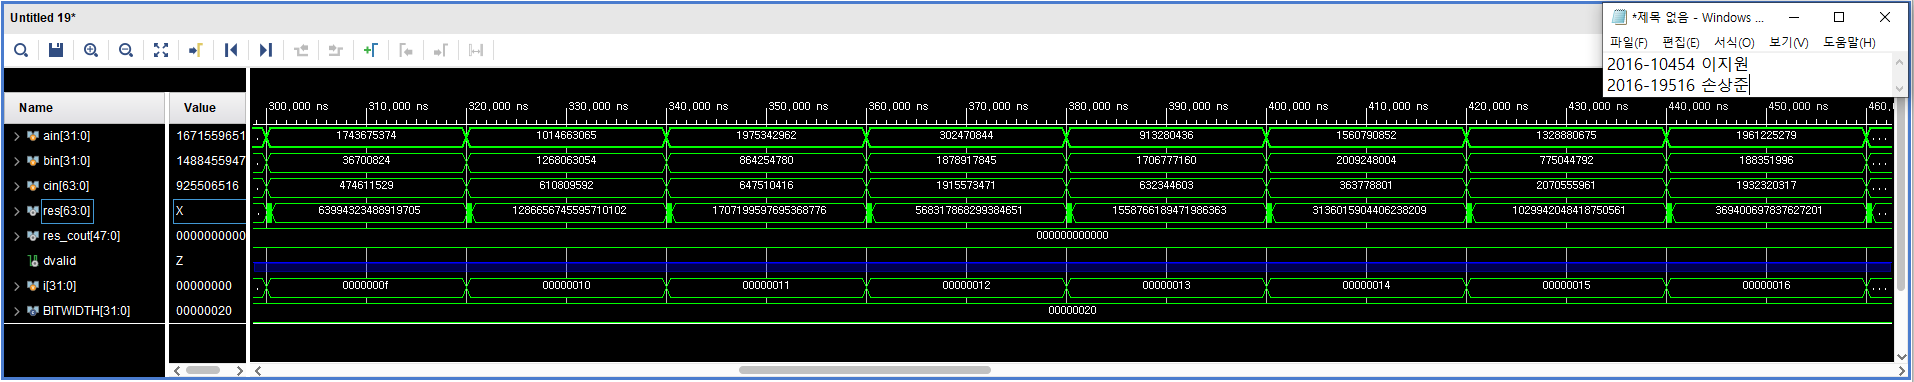
\includegraphics[width=1.0\textwidth]{../report/Waveform_32bit_Int_Multiply-Adder/tb_int_muladd3.png}
	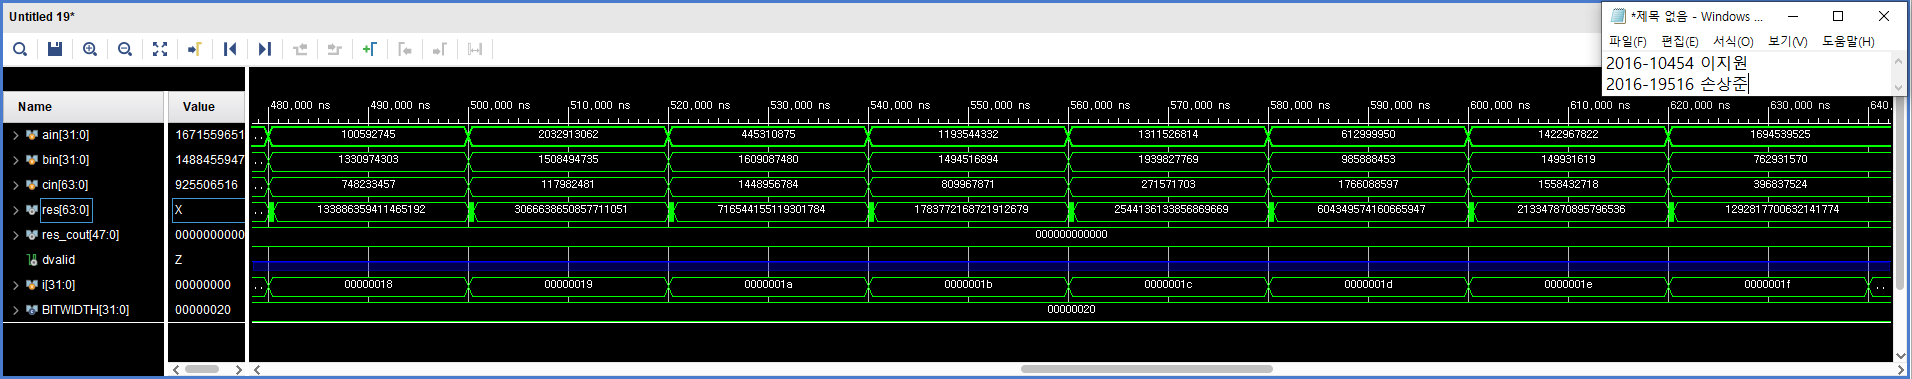
\includegraphics[width=1.0\textwidth]{../report/Waveform_32bit_Int_Multiply-Adder/tb_int_muladd4.png}
\end{figure}

\subsection{Adder-array}

\begin{lstlisting}[style={verilog-style}]
`timescale 1ns / 1ps
module my_add #(
    parameter BITWIDTH = 32
)
(
    input [BITWIDTH-1:0] ain,
    input [BITWIDTH-1:0] bin,
    output [BITWIDTH-1:0] dout,
    output overflow
);
    // concatnate (overflow, dout) & detect overflow
    assign {overflow, dout} = ain + bin;
endmodule
\end{lstlisting}

상기된 모듈은 Lab03 adder 모듈이다. ain과 bin 길이의 입력값이 주어지면 dout에 합산한 결과, overflow가 일어났을 경우를 판단하는 변수를 함께 전달해 주는 역할을 한다. Adder array의 구현은 generate-for statement를 사용하여 구현하였다. generate 구문에서는 다른 모듈의 instance를 선언할 수 있는데, 이번 과제에서는 Adder 모듈을 사용하여 출력값을 계산하였기 때문에, generate statement를 이용하였다.

cmd값이 바뀌게 되면, 출력값이 바로 바뀌어야 하기 때문에, 미리 모든 출력값을 계산한 후, cmd값에 따라 삼항연산자를 사용, multiplexer와 비슷하게 지정된 출력값만 출력되도록 설정하였다.

\begin{figure}[ht]
	\centering
	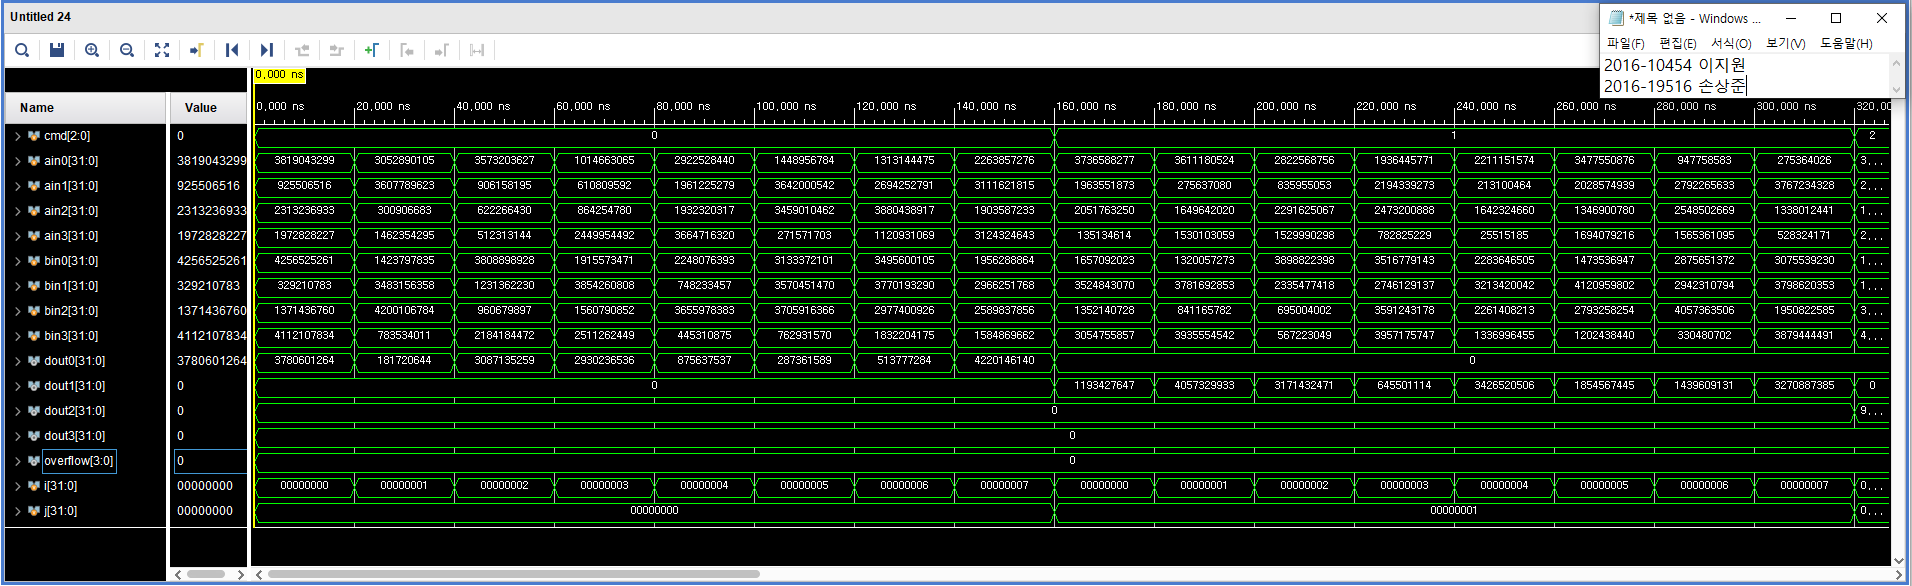
\includegraphics[width=1.0\textwidth]{../report/Waveform_Adder-Array/tb_adder_array1.png}
	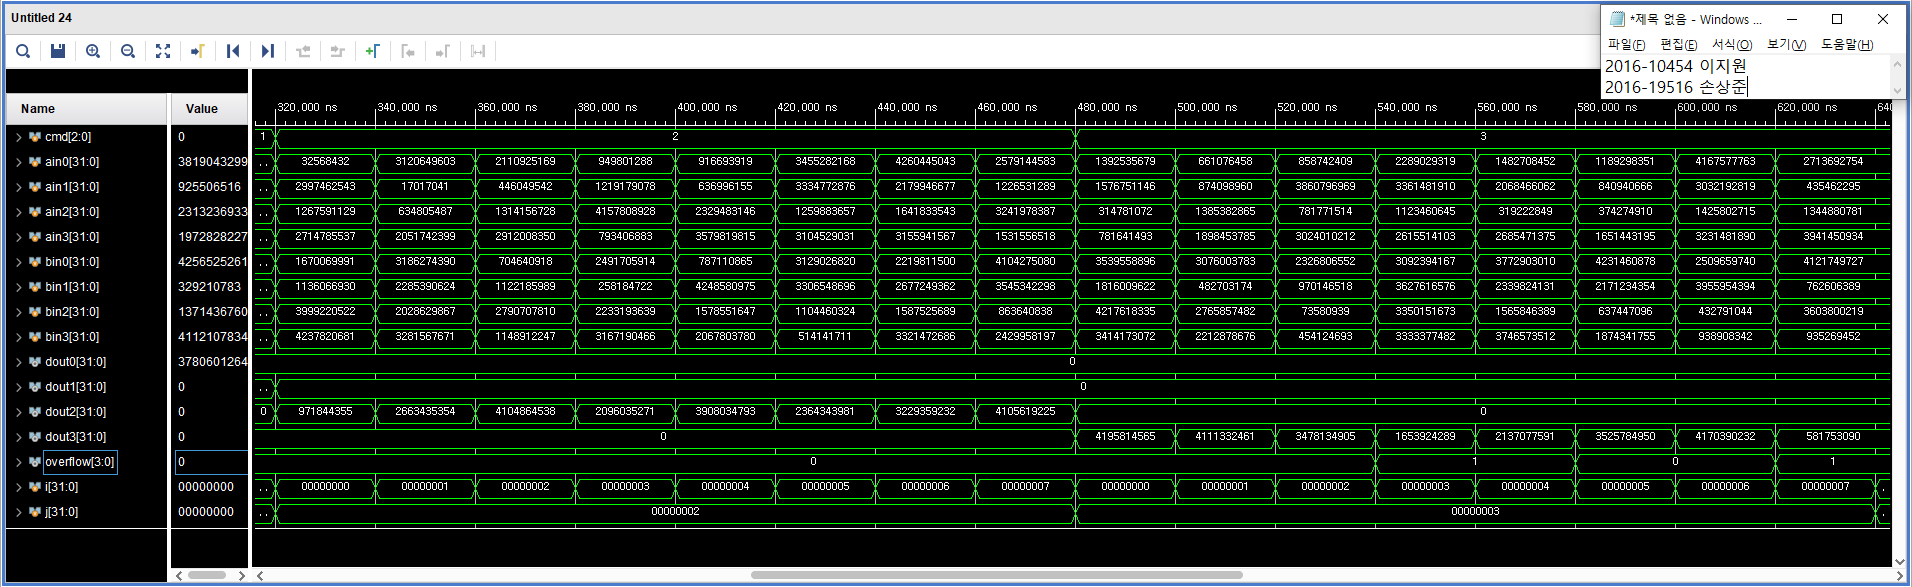
\includegraphics[width=1.0\textwidth]{../report/Waveform_Adder-Array/tb_adder_array2.png}
\end{figure}
 
\section{Conclusion}

입력되는 범위의 값들은 uniformly random하게 선택한 값들을 가지고 시뮬레이션 결과를 살펴보았을 때,
연산결과 값이 실제 값과 일치하는 것을 확인할 수 있었다.
Array를 이용하여 generate-for statement에서 간편하게 원하는 값을 얻어낸다는 점이 이번 프로젝트 구현 중 핵심 아이디어였다. 

cmd의 값에 따라 출력값을 변화시키기 위해 always @(cmd) 구문을 사용하지 않고, 삼항연산자를 사용할 때에도 원하는 형태로 waveform이 출력되었는데, 삼항연산자 자체도 always와 비슷한 역할로 event가 발생하면 출력값을 변화시키는 역할을 확인하였다.
향후 프로젝트에서 IP catalog를 이용해 기존의 모듈을 효율적으로 활용하여 코드를 작성하는 방법을 익힐 수 있었으며, custom modularization 과정을 익힐 수 있었다.
\newpage
\bibliographystyle{plain}
\bibliography{other}

\end{document}
